\documentclass[xcolor=dvipsnames]{beamer} % dvipsnames gives more built-in colors
\usepackage{graphicx}
\usetheme{Luebeck}
\useoutertheme{infolines} % Alternatively: miniframes, infolines, split
\useinnertheme{circles}
\usepackage{subcaption}
\usepackage{listings}
\usepackage{tikz,tikz-3dplot}
\usetikzlibrary{calc,arrows}
\usepackage{xcolor}
\lstset{
	basicstyle=\ttfamily\tiny,
	basewidth=0.65em,
	commentstyle=\ttfamily,
	tabsize=2,
	keywordstyle=\bfseries\sffamily,
	showstringspaces=false,
	numberstyle=\tiny,
	numbersep=2.5pt,
	keywordstyle=\bfseries\ttfamily,
	breaklines=true
}
\lstnewenvironment{pseudoc}{\lstset{frame=lines,mathescape=true, language = C++, basicstyle=\ttfamily\small, basewidth=0.55em}}{}

\definecolor{UBCblue}{rgb}{0.04706, 0.13725, 0.26667} % UBC Blue (primary)

\usecolortheme[named=MidnightBlue]{structure}
%\usecolortheme[named=Mahogany]{structure} % Sample dvipsnames color

\title[Valutazione del Contatto Pneumatico/Strada]{Valutazione Real-Time del Contatto Pneumatico/Strada con Algoritmi Dedicati}
\date{}

\usepackage{fontspec}
\defaultfontfeatures{Mapping=tex-text}
\setromanfont[Ligatures={Common}]{Adobe Caslon Pro}
\usefonttheme{serif}

\begin{document}

\begin{frame}
	\vspace{-.5cm}
	\titlepage
	\vspace{-2.5cm}
	\begin{center}
		\begin{tabular}{cc}
			\begin{minipage}[t]{0.45\textwidth}
				Relatore:\\
				\textbf{Prof. Enrico Bertolazzi}\\
				Università di Trento\\[.3cm]
				Co-relatore:\\
				\textbf{Dott. Ing. Matteo Ragni}\\
				AnteMotion S.r.l
			\end{minipage}
			& 
			\begin{minipage}[t]{0.45\textwidth}
				\begin{flushright}
					Candidato:\\
					\textbf{Davide Stocco}
				\end{flushright}
			\end{minipage}
		\end{tabular}
	\end{center}
	\begin{figure}
		\centering
		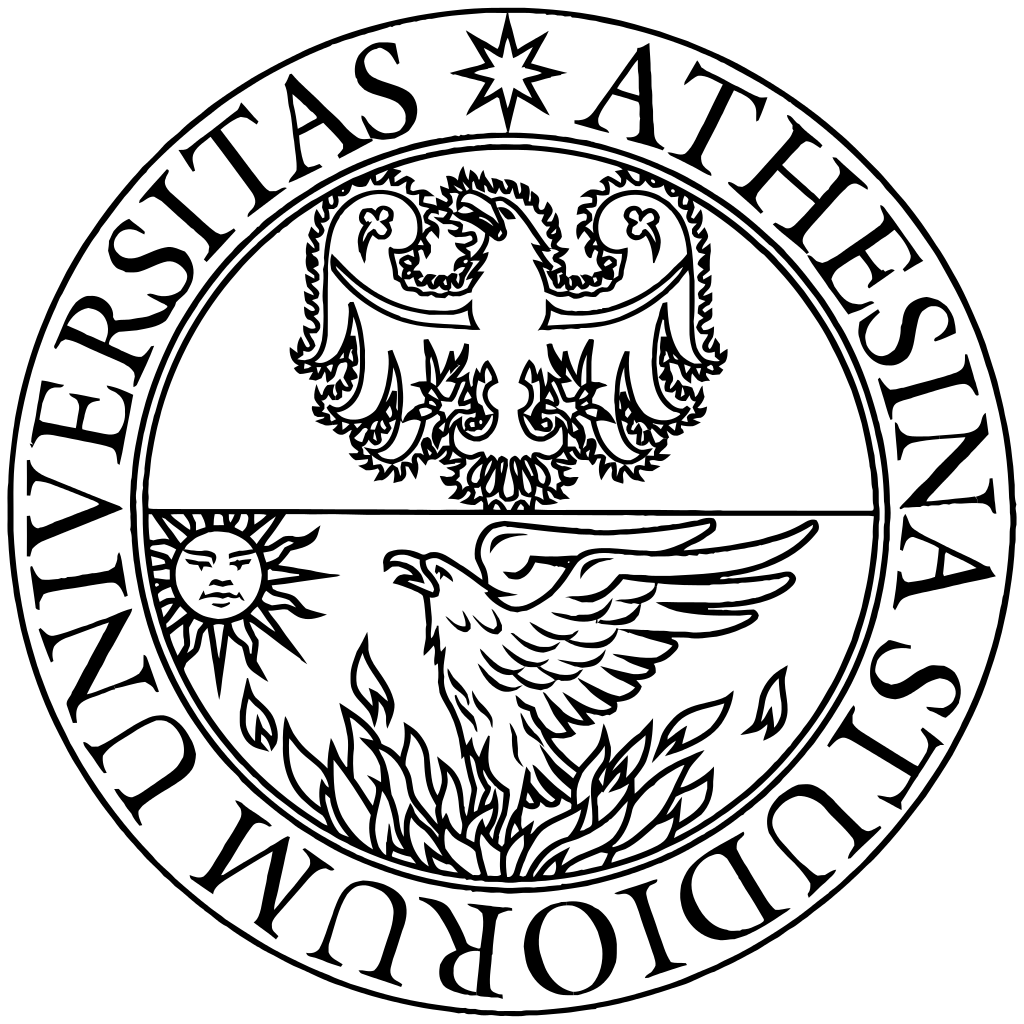
\includegraphics[width=0.15\linewidth]{../Figures/unitn}
	\end{figure}
\end{frame}

\author{Davide Stocco}

\begin{frame}
	\begin{figure}
		\centering
		
\includegraphics[width=0.5\linewidth]{../Figures/ante}
	\end{figure}
	\Large{\textbf{Motivazioni della Tesi}}
	\normalsize
	\begin{enumerate}
		\item Simulatore con
		\begin{enumerate}
			\item[$-$] \textit{Software in the Loop} (SIL)
			\item[$-$] \textit{Hardware in the Loop} (HIL)
			\item[$-$] \textit{Driver in	the Loop} (DIL)
		\end{enumerate}
		per la validazione degli \textit{Advanced Driver-Assistance Systems} (ADAS)
		\item \textbf{Valutazione del contatto pneumatico/strada}
	\end{enumerate}
\end{frame}
	
\begin{frame}
	\Large{\textbf{Obiettivi della Tesi}}
	\normalsize
	\begin{enumerate}
		\item Sviluppo di una libreria \texttt{C++} per la valutazione del contatto pneumatico/strada
		\item Applicazione in tempo reale
	\end{enumerate}
	\begin{figure}
		\centering
		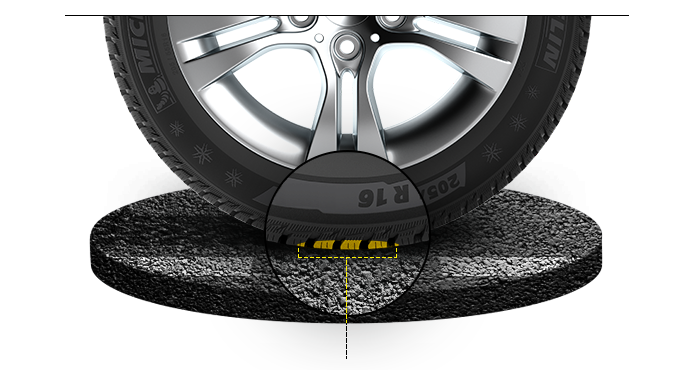
\includegraphics[width=0.6\linewidth]{../Figures/contact}
	\end{figure}
\end{frame}

\begin{frame}
	\Large{\textbf{Intersezione pneumatico/\textit{mesh}}}
	\normalsize
	\begin{enumerate}
		\item Analisi sintattico-grammaticale del formato \texttt{rdf}
		\item Istanziamento della \textit{mesh}
		\item Istanziamento dello pneumatico
		\item Posizionemanto dello pneumatico nello spazio
		\item Intersezione degli alberi AABB per trovare i triangoli candidati
		\item Scelta del modello di contatto
		\item Utilizzazione di algoritmi di tipo geometrico per valutare il contatto
		\item Estrazione dei risultati
	\end{enumerate}
\end{frame}

\begin{frame}[fragile]
	\Large{\textbf{Il formato \texttt{rdf} per le superfici stradali}}
	\normalsize
	\begin{figure}
		\centering
		\begin{subfigure}{\linewidth}
\begin{pseudoc}
[NODES]
{ id x_coord y_coord z_coord }
0 2.64637 35.8522 -1.59419e-005 
1 4.54089 33.7705 -1.60766e-005 
2 4.52126 35.8761 -1.62482e-005 
3 2.66601 33.7456 -1.57714e-005 
4 0.771484 35.8282 -1.56367e-005 
... ... ... ...
[ELEMENTS]
{ n1 n2 n3 mu }
1 2 3 1.0 
2 1 4 1.0 
... ... ... ...
\end{pseudoc}
		\end{subfigure}
	\end{figure}
%Altri parametri non considerati: \texttt{X\_SCALE}, \texttt{Z\_SCALE}, \texttt{Z\_SCALE}, \texttt{ORIGIN}, \texttt{ORIGIN} e \texttt{ORIENTATION}.
\end{frame}

\begin{frame}[fragile]
	\Large{\textbf{Analisi sintattico-grammaticale del formato \texttt{rdf}}}
	\normalsize
	\begin{enumerate}
		\item Estrazione dei \texttt{[NODES]}
		\item Estrazione degli \texttt{[ELEMENTS]}
		\item Istanziamento dei triangoli componenti la \textit{mesh}
		\item[$\textcolor{red}{\textbf{!!!}}$] \textcolor{red}{\textbf{Non esiste uno \textit{standard} per questo formato}}
	\end{enumerate}
\vspace{-0.3cm}
\begin{figure}
	\centering
	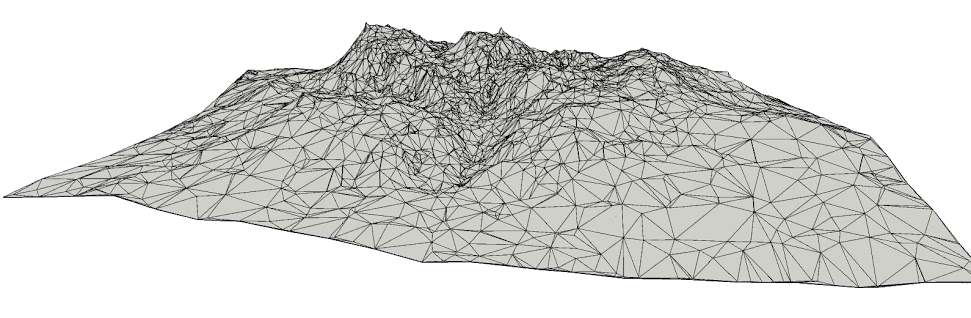
\includegraphics[width=0.7\linewidth]{../Figures/mesh}
\end{figure}
\vspace{-0.6cm}
\Large{\textbf{Istanziamento della \textit{mesh}}}
\begin{pseudoc}
TireGround::RDF::MeshSurface Road(
"./file.rdf" // Path to the *.rdf file
);
\end{pseudoc}
\end{frame}

\begin{frame}
	\Large{\textbf{Albero delle \textit{Axis-Aligned Bounding Boxes} (AABB)}}
	\normalsize
	\begin{enumerate}
		\item Raggruppamento ricorsivo delle AABB dei triangoli della \textit{mesh}
		\item Diminuzione in scala logaritmica del numero di comparazioni
		\item Solo confronti logici
	\end{enumerate}
	\begin{figure}
		\centering
		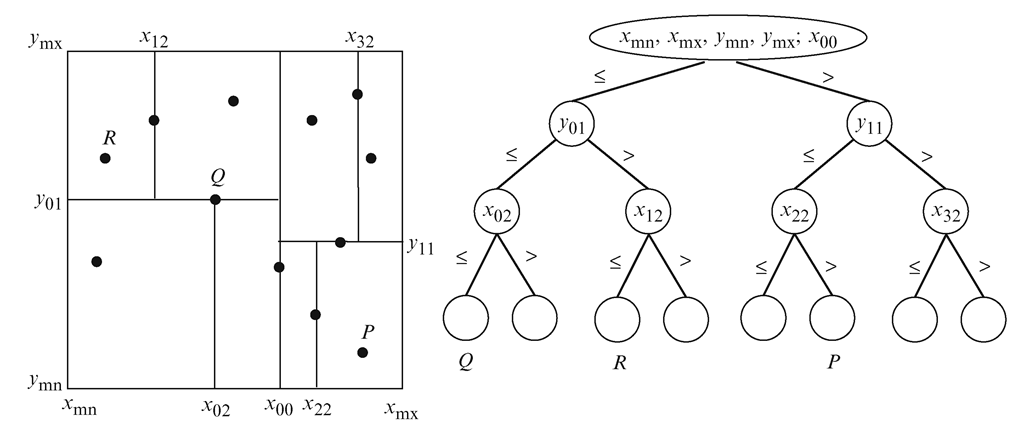
\includegraphics[width=0.85\linewidth]{../Figures/AABB}
	\end{figure}
\end{frame}

\begin{frame}
	\Large{\textbf{Modellizzazione geometrica dello pneumatico}}\\
	\normalsize
	Ente normatore: \textit{European Tire and Rim Technical Organization} (ETRTO)
	\begin{figure}
		\centering
		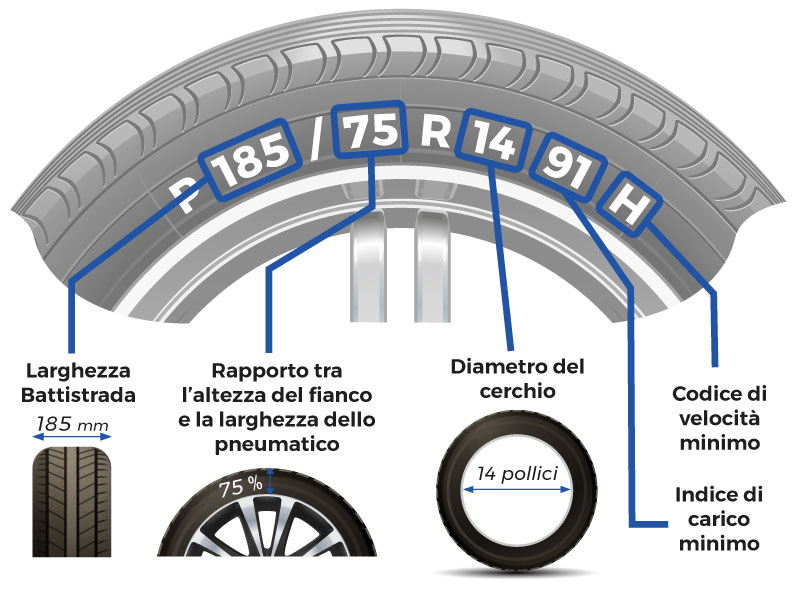
\includegraphics[width=0.7\linewidth]{../Figures/tire_measures}
	\end{figure}
\end{frame}

\begin{frame}
	\Large{\textbf{Rappresentazione dello pneumatico tramite dischi}}
	\normalsize
	\begin{enumerate}
		\item Uno o più dischi indeformabili
		\item Movimenti relativi consentiti
	\end{enumerate}
	\vspace{-.5cm}
	\begin{figure}
		\hfill
		\begin{subfigure}{0.45\linewidth}
			\centering
			\tdplotsetmaincoords{70}{110}
			\tdplotsetrotatedcoords{90}{90}{0}
			\begin{tikzpicture}[tdplot_main_coords,scale=0.6]	
			\draw[-stealth] (0,0,0) -- (8,0,0) node[anchor=north east]{$x_C$};
			\draw[-stealth] (0,0,0) -- (0,3,0) node[anchor=west]{$y_C$};
			\draw[-stealth] (0,0,0) -- (0,0,5) node[anchor=west]{$z_C$};
			\def\r{4};
			
			\begin{scope}[tdplot_rotated_coords]
			\tdplotdrawarc[tdplot_rotated_coords,thick]{(0,0,0)}{\r}{0}{360}{}{}
			\end{scope}
			\end{tikzpicture}
			\small{Disco singolo}
		\end{subfigure}
		\hfill
		\begin{subfigure}{0.45\linewidth}
			\centering
			\tdplotsetmaincoords{70}{110}
			\tdplotsetrotatedcoords{90}{90}{0}
			\begin{tikzpicture}[tdplot_main_coords,scale=0.6]
				\draw[-stealth] (0,0,0) -- (9,0,0) node[anchor=north east]{$x_C$};
				\draw[-stealth] (0,0,0) -- (0,3.5,0) node[anchor=west]{$y_C$};
				\draw[-stealth] (0,0,0) -- (0,0,5) node[anchor=west]{$z_C$};
				\def\r{4};
				
				\begin{scope}[tdplot_rotated_coords]
				\tdplotdrawarc[tdplot_rotated_coords,thick]{(0,0,1.6)}{\r-0.5}{0}{360}{}{}
				
				\tdplotdrawarc[tdplot_rotated_coords,thick]{(0,0,1.2)}{\r-0.5+0.5*1.41/2}{3}{-228}{}{}
				\tdplotdrawarc[tdplot_rotated_coords, dashed,thick]{(0,0,1.2)}{\r-0.5+0.5*1.41/2}{3}{360-228}{}{}
				
				\tdplotdrawarc[tdplot_rotated_coords,thick]{(0,0,0.8)}{\r}{-9}{-217}{}{}
				\tdplotdrawarc[tdplot_rotated_coords, dashed,thick]{(0,0,0.8)}{\r}{-9}{360-217}{}{}
				
				\tdplotdrawarc[tdplot_rotated_coords,thick]{(0,0,0.4)}{\r}{-15}{-210}{}{}
				\tdplotdrawarc[tdplot_rotated_coords, dashed,thick]{(0,0,0.4)}{\r}{-15}{360-210}{}{}
				
				\tdplotdrawarc[tdplot_rotated_coords,thick]{(0,0,0)}{\r}{-15}{-210}{}{}
				\tdplotdrawarc[tdplot_rotated_coords, dashed,thick]{(0,0,0)}{\r}{-15}{360-210}{}{}
				
				\tdplotdrawarc[tdplot_rotated_coords,thick]{(0,0,-0.4)}{\r}{-15}{-210}{}{}
				\tdplotdrawarc[tdplot_rotated_coords, dashed,thick]{(0,0,-0.4)}{\r}{-15}{360-210}{}{}
				
				\tdplotdrawarc[tdplot_rotated_coords,thick]{(0,0,-0.8)}{\r}{-15}{-210}{}{}
				\tdplotdrawarc[tdplot_rotated_coords, dashed,thick]{(0,0,-0.8)}{\r}{-15}{360-210}{}{}
				
				\tdplotdrawarc[tdplot_rotated_coords,thick]{(0,0,-1.2)}{\r-0.5+0.5*1.41/2}{-17}{-205}{}{}
				\tdplotdrawarc[tdplot_rotated_coords, dashed,thick]{(0,0,-1.2)}{\r-0.5+0.5*1.41/2}{-17}{360-205}{}{}
				
				\tdplotdrawarc[tdplot_rotated_coords,thick]{(0,0,-1.6)}{\r-0.5}{-30}{-195}{}{}
				\tdplotdrawarc[tdplot_rotated_coords, dashed,thick]{(0,0,-1.6)}{\r-0.5}{-20}{360-195}{}{}
				\end{scope}
			\end{tikzpicture}
			\small{Dischi multipli}
		\end{subfigure}
	\hfill
	\end{figure}
\vspace{-.5cm}
\end{frame}

\begin{frame}
	\Large{\textbf{Disposizione dei dischi}}
	\normalsize
	\begin{figure}[h!]
		\hfill
		\begin{subfigure}{.3\textwidth}
			\centering
			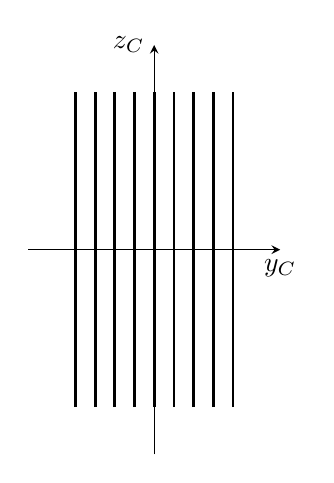
\begin{tikzpicture}
			\def\axisl{2};
			\def\zd{1};
			\draw[-stealth] (-0.8*\axisl,0) -- (0.8*\axisl,0) node[below]{$y_C$};
			\draw[-stealth] (0,-1.3*\axisl) -- (0,1.3*\axisl) node[left]{$z_C$};
			
			\draw[line width=0.35mm] (-1,-\axisl/\zd) -- (-1,\axisl/\zd);
			\draw[line width=0.35mm] (-0.75,-\axisl/\zd) -- (-0.75,\axisl/\zd);
			\draw[line width=0.35mm] (-0.5,-\axisl/\zd) -- (-0.5,\axisl/\zd);
			\draw[line width=0.35mm] (-0.25,-\axisl/\zd) -- (-0.25,\axisl/\zd);
			
			\draw[line width=0.35mm] (0,-\axisl/\zd) -- (0,\axisl/\zd);
			
			\draw[line width=0.35mm] (0.25,-\axisl/\zd) -- (0.25,\axisl/\zd);
			\draw[line width=0.35mm] (0.5,-\axisl/\zd) -- (0.5,\axisl/\zd);
			\draw[line width=0.35mm] (0.75,-\axisl/\zd) -- (0.75,\axisl/\zd);
			\draw[line width=0.35mm] (1,-\axisl/\zd) -- (1,\axisl/\zd);
			\end{tikzpicture}
			\small{Raggio uniforme}
		\end{subfigure}
		\hfill
		\begin{subfigure}{.3\textwidth}
			\centering
			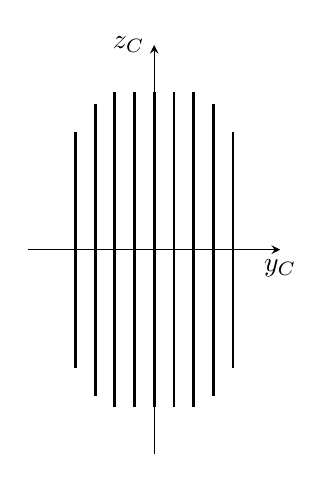
\begin{tikzpicture}
			\def\axisl{2};
			\def\zd{1};
			\draw[-stealth] (-0.8*\axisl,0) -- (0.8*\axisl,0) node[below]{$y_C$};
			\draw[-stealth] (0,-1.3*\axisl) -- (0,1.3*\axisl) node[left]{$z_C$};
			
			\draw[line width=0.35mm] (-1,-\axisl/\zd+0.5) -- (-1,\axisl/\zd-0.5);
			\draw[line width=0.35mm] (-0.75,-\axisl/\zd+0.5-0.5*1.41/2) -- (-0.75,\axisl/\zd-0.5+0.5*1.41/2);
			\draw[line width=0.35mm] (-0.5,-\axisl/\zd) -- (-0.5,\axisl/\zd);
			\draw[line width=0.35mm] (-0.25,-\axisl/\zd) -- (-0.25,\axisl/\zd);
			
			\draw[line width=0.35mm] (0,-\axisl/\zd) -- (0,\axisl/\zd);
			
			\draw[line width=0.35mm] (0.25,-\axisl/\zd) -- (0.25,\axisl/\zd);
			\draw[line width=0.35mm] (0.5,-\axisl/\zd) -- (0.5,\axisl/\zd);
			\draw[line width=0.35mm] (0.75,-\axisl/\zd+0.5-0.5*1.41/2) -- (0.75,\axisl/\zd-0.5+0.5*1.41/2);
			\draw[line width=0.35mm] (1,-\axisl/\zd+0.5) -- (1,\axisl/\zd-0.5);
			\end{tikzpicture}
			\small{Spalla raccordata}
		\end{subfigure}
		\hfill
		\begin{subfigure}{.3\textwidth}
			\centering
			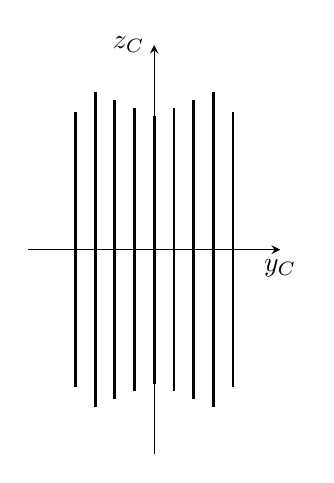
\begin{tikzpicture}
			\def\axisl{2};
			\def\zd{1};
			\draw[-stealth] (-0.8*\axisl,0) -- (0.8*\axisl,0) node[below]{$y_C$};
			\draw[-stealth] (0,-1.3*\axisl) -- (0,1.3*\axisl) node[left]{$z_C$};
			
			\draw[line width=0.35mm] (-1,-\axisl/\zd+0.25) -- (-1,\axisl/\zd-0.25);
			\draw[line width=0.35mm] (-0.75,-\axisl/\zd) -- (-0.75,\axisl/\zd);
			\draw[line width=0.35mm] (-0.5,-\axisl/\zd+0.1) -- (-0.5,\axisl/\zd-0.1);
			\draw[line width=0.35mm] (-0.25,-\axisl/\zd+0.2) -- (-0.25,\axisl/\zd-0.2);
			
			\draw[line width=0.35mm] (0,-\axisl/\zd+0.3) -- (0,\axisl/\zd-0.3);
			
			\draw[line width=0.35mm] (0.25,-\axisl/\zd+0.2) -- (0.25,\axisl/\zd-0.2);
			\draw[line width=0.35mm] (0.5,-\axisl/\zd+0.1) -- (0.5,\axisl/\zd-0.1);
			\draw[line width=0.35mm] (0.75,-\axisl/\zd) -- (0.75,\axisl/\zd);
			\draw[line width=0.35mm] (1,-\axisl/\zd+0.25) -- (1,\axisl/\zd-0.25);
			\end{tikzpicture}
			\small{Profilo personalizzato}
		\end{subfigure}
		\hfill
	\end{figure}
\end{frame}

\begin{frame}[fragile]
	\Large{\textbf{Istanziamento dello pneumatico}}
	\normalsize
\begin{pseudoc}
TireGround::Tire* TireSD = new TireGround::MagicFormula(
SectionWidth, // [m]
AspectRatio,  // [%]
RimDiameter,  // [in]
SwitchNumber  // Max triangles in the shadow
);
\end{pseudoc}
\begin{pseudoc}
TireGround::Tire* TireMD = new TireGround::MultiDisk(
SectionWidth, // [m]
AspectRatio,  // [%]
RimDiameter,  // [in]
RadiusVec,    // Disks radius vector [m]
PointsNumber, // Sampling points for each disk
SwitchNumber  // Max triangles in the shadow
);
\end{pseudoc}
\end{frame}

\begin{frame}
	\Large{\textbf{Modelli di contatto per pneumatico mono-disco}}
	\normalsize
	\begin{enumerate}
		\item Modello di contatto di Rill
	\end{enumerate}
\begin{figure}
	\centering
	\begin{subfigure}{\linewidth}
		\centering
		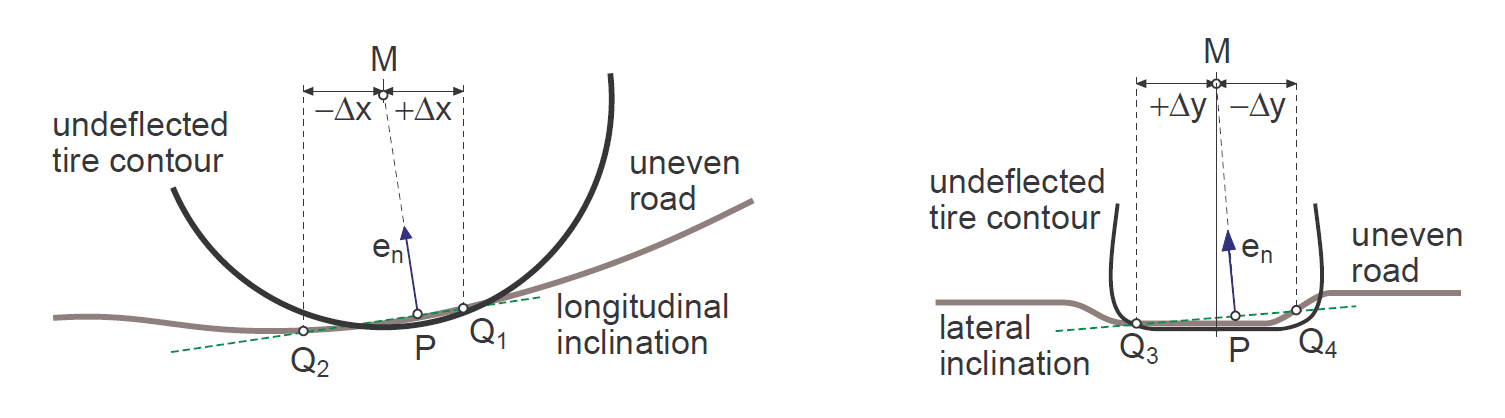
\includegraphics[width=0.8\linewidth]{../Figures/local_plane_1}
	\end{subfigure}\\
	\begin{subfigure}{0.45\linewidth}
		\centering
		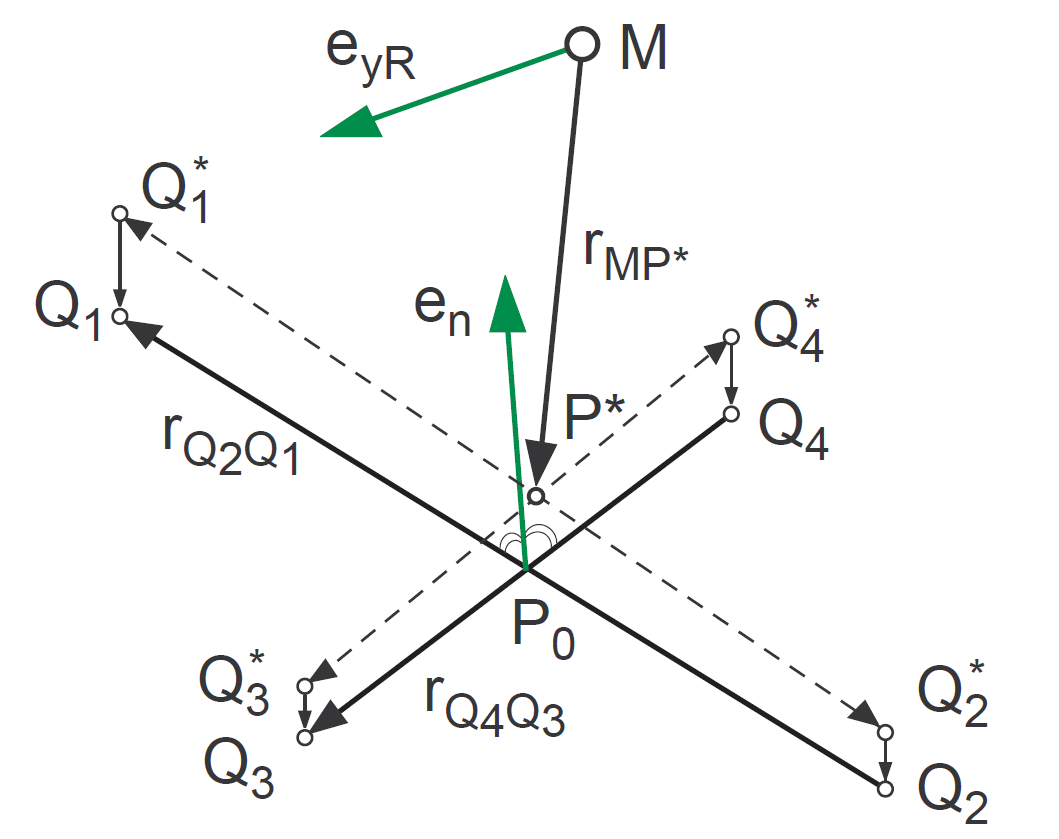
\includegraphics[width=0.7\linewidth]{../Figures/local_track}
	\end{subfigure}
	\begin{subfigure}{0.45\linewidth}
		\centering
		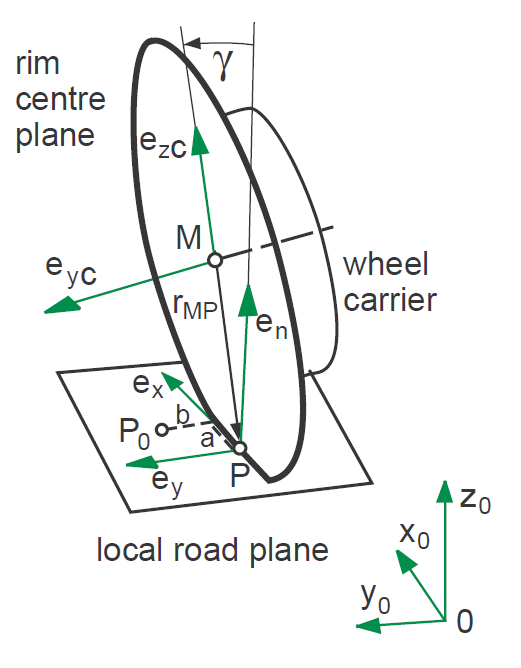
\includegraphics[width=0.5\linewidth]{../Figures/contact_geometry_2}
	\end{subfigure}
\end{figure}
		
\end{frame}

\begin{frame}
	\begin{enumerate}\addtocounter{enumi}{1}
		\item Modello di contatto ponderato in base all'area d'intersezione
	\end{enumerate}
	\begin{figure}
	\centering
	\hfill
		\begin{subfigure}{0.45\linewidth}
			\centering
			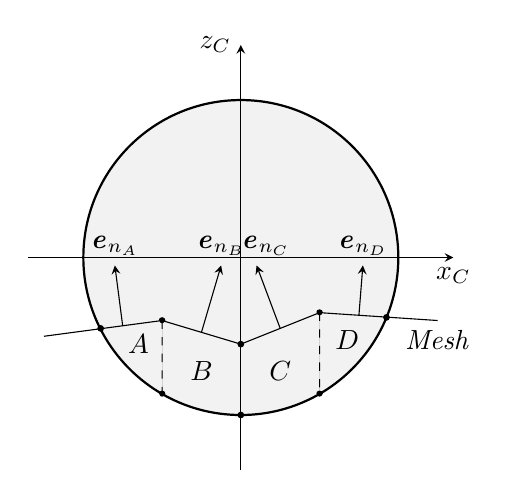
\begin{tikzpicture}[scale=1]
			\def\axisl{2.7};
			\def\zd{1.9};
			\draw[thick, fill=gray!10] (0,0) circle (2);
			\draw[-stealth] (-\axisl,0) -- (\axisl,0) node[below]{$x_C$};
			\draw[-stealth] (0,-\axisl) -- (0,\axisl) node[left]{$z_C$};
			\draw[] (-2.5,-1)  -- (-1,-0.8) --  (0,-1.1) -- (1,-0.7) -- (2.5,-0.8) node[below]{\textit{Mesh}};
			\draw[fill] (0,-1.1) circle [radius=1pt];
			\draw[fill] (0,-2) circle [radius=1pt];
			\draw[fill] (-1.78,-0.9) circle [radius=1pt];
			\draw[fill] (1.85,-0.76) circle [radius=1pt];
			\draw[dashed, fill] (-1,-0.8)  circle [radius=1pt] --  (-1,-2*0.866)  circle [radius=1pt];
			\draw[dashed, fill] (1,-0.7)  circle [radius=1pt] --  (1,-2*0.866)  circle [radius=1pt];
			\draw[]  (1.35,-0.8) node[below]{$D$};
			\draw[]  (0.5,-1.2) node[below]{$C$};
			\draw[]  (-0.5,-1.2) node[below]{$B$};
			\draw[]  (-1.3,-0.85) node[below]{$A$};
			\draw[-stealth] (1.5,-0.73) -- (1.55,-0.1) node[above]{$\textbf{\textit{e}}_{n_D}$};
			\draw[-stealth] (0.5,-0.9)  -- (0.2,-0.1) node[above]{$~~\textbf{\textit{e}}_{n_C}$};
			\draw[-stealth] (-0.5,-0.95) -- (-0.25,-0.1) node[above]{$\textbf{\textit{e}}_{n_B}$};
			\draw[-stealth] (-1.5,-0.87) -- (-1.6,-0.1) node[above]{$\textbf{\textit{e}}_{n_A}$};
			\end{tikzpicture}
		\end{subfigure}
	\hfill
		\begin{subfigure}{0.45\linewidth}
			\centering
			\tdplotsetmaincoords{70}{110}
			\tdplotsetrotatedcoords{90}{90}{0}
			\begin{tikzpicture}[tdplot_main_coords,scale=0.65]
			
			\draw[-stealth] (0,0,0) -- (7,0,0) node[anchor=north east]{$x_C$};
			\draw[-stealth] (0,0,0) -- (0,2.5,0) node[anchor=north west]{$y_C$};
			\draw[-stealth] (0,0,0) -- (0,0,5) node[anchor=south]{$z_C$};
			
			\def\r{4};
			
			\draw[-stealth,blue,very thick] (0,0,-\r) -- (0,0.1,-\r+1.5);
			
			\begin{scope}[tdplot_rotated_coords]
			\tdplotdrawarc[tdplot_rotated_coords,thick]{(0,0,0)}{\r}{0}{360}{}{}
			\end{scope}
			\end{tikzpicture}
		\end{subfigure}
	\hfill
	\end{figure}
\end{frame}

\begin{frame}
	\Large{\textbf{Differenze tra le due tipologie di modelli di contatto}}
	\normalsize
	\begin{figure}
		\centering
		\hfill
		\begin{subfigure}[t]{0.45\linewidth}
			\centering
			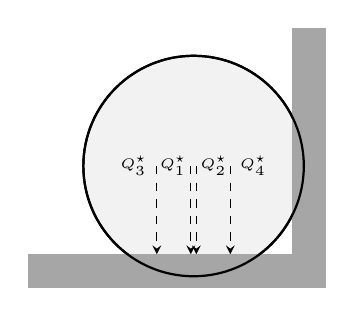
\begin{tikzpicture}[scale=0.7]
			\def\axisl{3};
			\def\zd{3.5};
			\draw[thick, fill=gray!10] (0,0) circle (2);
			\draw[-stealth, dashed] (-2/3,0) node[left]{\tiny$Q^\star_3$}-- (-2/3,-1.6);
			\draw[-stealth, dashed] (2/3,0) node[right]{\tiny$Q^\star_4$} -- (2/3,-1.6) ;
			\draw[-stealth, dashed] (0.05,0) node[left]{\tiny$Q^\star_1$}-- (0.05,-1.6);
			\draw[-stealth, dashed] (-0.05,0) node[right]{\tiny$Q^\star_2$}-- (-0.05,-1.6);
			\draw[fill, gray!70] (-\axisl,-1.6) --  (1.8,-1.6)  -- (1.8,2.5) -- (2.4,2.5) -- (2.4,-2.2) -- (-\axisl,-2.2);
			\draw[thick] (0,0) circle (2);
			\end{tikzpicture}
			\\[0.1cm]
			Rill:
			\begin{itemize}
				\item[$-$] \textcolor{red}{\textbf{Non rileva ostacoli frontali}}
				\item[$-$] \textcolor{red}{\textbf{Approssimativo}}
			\end{itemize}
		\end{subfigure}
		\hfill
		\begin{subfigure}[t]{0.45\linewidth}
			\centering
			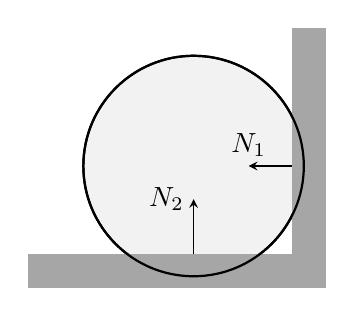
\begin{tikzpicture}[scale=0.7]
			\def\axisl{3};
			\def\zd{3.5};
			\draw[thick, fill=gray!10] (0,0) circle (2);
			\draw[-stealth] (1.8,0) -- (1,0) node[above]{$N_1$};
			\draw[-stealth] (0,-1.6) -- (0,-0.6) node[left]{$N_2$};
			\draw[fill, gray!70] (-\axisl,-1.6) --  (1.8,-1.6)  -- (1.8,2.5) -- (2.4,2.5) -- (2.4,-2.2) -- (-\axisl,-2.2);
			\draw[thick] (0,0) circle (2);	
			\end{tikzpicture}
			\\[0.1cm]
			Ponderato sull'area d'intersezione:
			\begin{itemize}
				\item[$+$] \textcolor{green}{\textbf{Rileva ostacoli frontali}}\\
				\item[$+$] \textcolor{green}{\textbf{Robusto se la \textit{mesh} ha "buchi"}}
				\item[$-$] \textcolor{red}{\textbf{Poco robusto se i triangoli sono sovrapposti}}				
			\end{itemize}
		\end{subfigure}
		\hfill
	\end{figure}
\end{frame}

\begin{frame}
	\Large{\textbf{Modelli di contatto per pneumatico multi-disco}}
	\normalsize
	\begin{enumerate}
		\item Modello di contatto ponderato in base all'area d'intersezione
	\end{enumerate}
	\begin{figure}
		\centering
		\hfill
		\begin{subfigure}{0.45\linewidth}
			\centering
			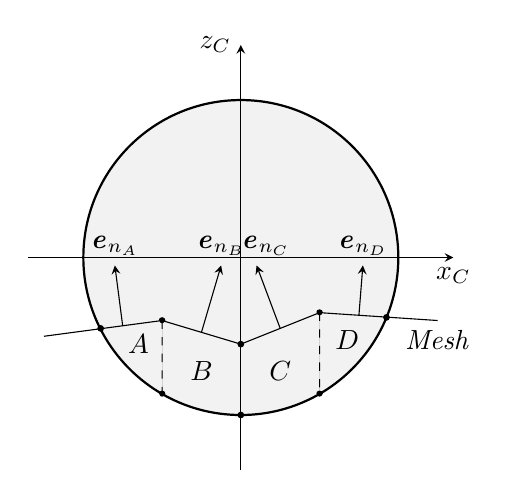
\begin{tikzpicture}[scale=1]
			\def\axisl{2.7};
			\def\zd{1.9};
			\draw[thick, fill=gray!10] (0,0) circle (2);
			\draw[-stealth] (-\axisl,0) -- (\axisl,0) node[below]{$x_C$};
			\draw[-stealth] (0,-\axisl) -- (0,\axisl) node[left]{$z_C$};
			\draw[] (-2.5,-1)  -- (-1,-0.8) --  (0,-1.1) -- (1,-0.7) -- (2.5,-0.8) node[below]{\textit{Mesh}};
			\draw[fill] (0,-1.1) circle [radius=1pt];
			\draw[fill] (0,-2) circle [radius=1pt];
			\draw[fill] (-1.78,-0.9) circle [radius=1pt];
			\draw[fill] (1.85,-0.76) circle [radius=1pt];
			\draw[dashed, fill] (-1,-0.8)  circle [radius=1pt] --  (-1,-2*0.866)  circle [radius=1pt];
			\draw[dashed, fill] (1,-0.7)  circle [radius=1pt] --  (1,-2*0.866)  circle [radius=1pt];
			\draw[]  (1.35,-0.8) node[below]{$D$};
			\draw[]  (0.5,-1.2) node[below]{$C$};
			\draw[]  (-0.5,-1.2) node[below]{$B$};
			\draw[]  (-1.3,-0.85) node[below]{$A$};
			\draw[-stealth] (1.5,-0.73) -- (1.55,-0.1) node[above]{$\textbf{\textit{e}}_{n_D}$};
			\draw[-stealth] (0.5,-0.9)  -- (0.2,-0.1) node[above]{$~~\textbf{\textit{e}}_{n_C}$};
			\draw[-stealth] (-0.5,-0.95) -- (-0.25,-0.1) node[above]{$\textbf{\textit{e}}_{n_B}$};
			\draw[-stealth] (-1.5,-0.87) -- (-1.6,-0.1) node[above]{$\textbf{\textit{e}}_{n_A}$};
			\end{tikzpicture}
		\end{subfigure}
		\hfill
		\begin{subfigure}{0.45\linewidth}
			\centering
			\tdplotsetmaincoords{70}{110}
			\tdplotsetrotatedcoords{90}{90}{0}
			\begin{tikzpicture}[tdplot_main_coords,scale=0.65]
			
			\draw[-stealth] (0,0,0) -- (9,0,0) node[anchor=north east]{$x_C$};
			\draw[-stealth] (0,0,0) -- (0,3.5,0) node[anchor=north west]{$y_C$};
			\draw[-stealth] (0,0,0) -- (0,0,5) node[anchor=south]{$z_C$};
			
			\def\r{4};
			\draw[-stealth,red] (0,1.6,-\r+0.5) -- (0,1.6,-\r+1.5);
			\draw[-stealth,red] (0,1.2,-\r+0.5-0.5*1.41/2) -- (0-0.1,1.2+0.1,-\r+1.5-0.5*1.41/2);
			\draw[-stealth,red] (0,0.8,-\r) -- (0,0.8,-\r+1);
			\draw[-stealth,red] (0,0.4,-\r) -- (0+0.1,0.4-0.1,-\r+1);
			\draw[-stealth,red] (0,0,-\r) -- (0+0.05,0-0.1,-\r+1);
			\draw[-stealth,red] (0,-0.4,-\r) -- (0,-0.4,-\r+1);
			\draw[-stealth,red] (0,-0.8,-\r) -- (0+0.1,-0.8+0.1,-\r+1);
			\draw[-stealth,red] (0,-1.2,-\r+0.5-0.5*1.41/2) -- (0,-1.2,-\r+1.5-0.5*1.41/2);
			\draw[-stealth,red] (0,-1.6,-\r+0.5) -- (0,-1.6,-\r+1.5);
			
			\draw[-stealth,blue,very thick] (0,0,-\r) -- (0,0,-\r+1.5);
			
			\begin{scope}[tdplot_rotated_coords]
			\tdplotdrawarc[tdplot_rotated_coords,thick]{(0,0,1.6)}{\r-0.5}{0}{360}{}{}
			
			\tdplotdrawarc[tdplot_rotated_coords,thick]{(0,0,1.2)}{\r-0.5+0.5*1.41/2}{3}{-228}{}{}
			\tdplotdrawarc[tdplot_rotated_coords, dashed,thick]{(0,0,1.2)}{\r-0.5+0.5*1.41/2}{3}{360-228}{}{}
			
			\tdplotdrawarc[tdplot_rotated_coords,thick]{(0,0,0.8)}{\r}{-9}{-217}{}{}
			\tdplotdrawarc[tdplot_rotated_coords, dashed,thick]{(0,0,0.8)}{\r}{-9}{360-217}{}{}
			
			\tdplotdrawarc[tdplot_rotated_coords,thick]{(0,0,0.4)}{\r}{-15}{-210}{}{}
			\tdplotdrawarc[tdplot_rotated_coords, dashed,thick]{(0,0,0.4)}{\r}{-15}{360-210}{}{}
			
			\tdplotdrawarc[tdplot_rotated_coords,thick]{(0,0,0)}{\r}{-15}{-210}{}{}
			\tdplotdrawarc[tdplot_rotated_coords, dashed,thick]{(0,0,0)}{\r}{-15}{360-210}{}{}
			
			\tdplotdrawarc[tdplot_rotated_coords,thick]{(0,0,-0.4)}{\r}{-15}{-210}{}{}
			\tdplotdrawarc[tdplot_rotated_coords, dashed,thick]{(0,0,-0.4)}{\r}{-15}{360-210}{}{}
			
			\tdplotdrawarc[tdplot_rotated_coords,thick]{(0,0,-0.8)}{\r}{-15}{-210}{}{}
			\tdplotdrawarc[tdplot_rotated_coords, dashed,thick]{(0,0,-0.8)}{\r}{-15}{360-210}{}{}
			
			\tdplotdrawarc[tdplot_rotated_coords,thick]{(0,0,-1.2)}{\r-0.5+0.5*1.41/2}{-17}{-205}{}{}
			\tdplotdrawarc[tdplot_rotated_coords, dashed,thick]{(0,0,-1.2)}{\r-0.5+0.5*1.41/2}{-17}{360-205}{}{}
			
			\tdplotdrawarc[tdplot_rotated_coords,thick]{(0,0,-1.6)}{\r-0.5}{-30}{-195}{}{}
			\tdplotdrawarc[tdplot_rotated_coords, dashed,thick]{(0,0,-1.6)}{\r-0.5}{-20}{360-195}{}{}
			\end{scope}
			\end{tikzpicture}
		\end{subfigure}
		\hfill
	\end{figure}
\end{frame}

\begin{frame}
	\begin{enumerate}\addtocounter{enumi}{1}
		\item Modello di contatto tramite campionamento
	\end{enumerate}
	\begin{figure}
		\centering
		\hfill
		\begin{subfigure}{0.45\linewidth}
			\centering
			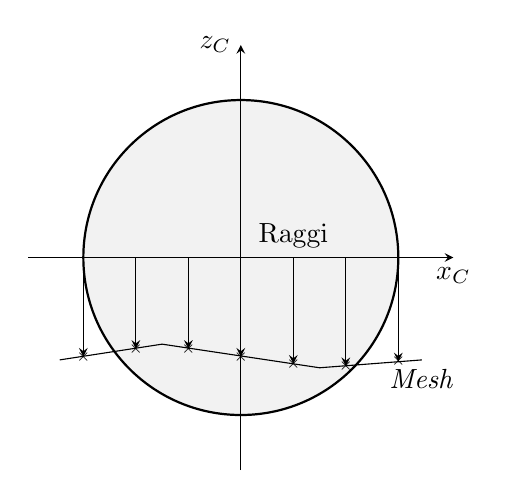
\begin{tikzpicture}
			\def\axisl{2.7};
			\def\zd{3.5};
			\draw[thick, fill=gray!10] (0,0) circle (2);
			\draw[-stealth] (-\axisl,0) -- (\axisl,0) node[below]{$x_C$};
			\draw[-stealth] (0,-\axisl) -- (0,\axisl) node[left]{$z_C$};
			\draw[-stealth] (-2,0) -- (-2,-1.26) node[]{\tiny$\times$};
			\draw[-stealth] (2,0) -- (2,-1.32) node[]{\tiny$\times$};
			\draw[-stealth] (-2*2/3,0) -- (-2*2/3,-1.16) node[]{\tiny$\times$};
			\draw[-stealth] (2*2/3,0) -- (2*2/3,-1.38) node[]{\tiny$\times$};
			\draw[-stealth] (-2/3,0) -- (-2/3,-1.16) node[]{\tiny$\times$};
			\draw[-stealth] (2/3,0) node[above]{Raggi} -- (2/3,-1.35) node[]{\tiny$\times$};
			\draw[-stealth] (0,0) -- (0,-1.26) node[]{\tiny$\times$};
			\draw[] (-2.3,-1.3) -- (-1,-1.1) --  (1,-1.4) -- (2.3,-1.3) node[below]{\textit{Mesh}};
			\end{tikzpicture}
		\end{subfigure}
		\hfill
		\begin{subfigure}{0.45\linewidth}
			\centering
			\tdplotsetmaincoords{70}{110}
			\tdplotsetrotatedcoords{90}{90}{0}
			\begin{tikzpicture}[tdplot_main_coords,scale=0.65]
			
			\draw[-stealth] (0,0,0) -- (9,0,0) node[anchor=north east]{$x_C$};
			\draw[-stealth] (0,0,0) -- (0,3.5,0) node[anchor=north west]{$y_C$};
			\draw[-stealth] (0,0,0) -- (0,0,5) node[anchor=south]{$z_C$};
			
			\def\r{4};
			\draw[-stealth,red] (0,1.6,-\r+0.5) -- (0,1.6,-\r+1.5);
			\draw[-stealth,red] (0,1.2,-\r+0.5-0.5*1.41/2) -- (0-0.1,1.2+0.1,-\r+1.5-0.5*1.41/2);
			\draw[-stealth,red] (0,0.8,-\r) -- (0,0.8,-\r+1);
			\draw[-stealth,red] (0,0.4,-\r) -- (0+0.1,0.4-0.1,-\r+1);
			\draw[-stealth,red] (0,0,-\r) -- (0+0.05,0-0.1,-\r+1);
			\draw[-stealth,red] (0,-0.4,-\r) -- (0,-0.4,-\r+1);
			\draw[-stealth,red] (0,-0.8,-\r) -- (0+0.1,-0.8+0.1,-\r+1);
			\draw[-stealth,red] (0,-1.2,-\r+0.5-0.5*1.41/2) -- (0,-1.2,-\r+1.5-0.5*1.41/2);
			\draw[-stealth,red] (0,-1.6,-\r+0.5) -- (0,-1.6,-\r+1.5);
			
			\draw[-stealth,blue,very thick] (0,0,-\r) -- (0,0,-\r+1.5);
			
			\begin{scope}[tdplot_rotated_coords]
			\tdplotdrawarc[tdplot_rotated_coords,thick]{(0,0,1.6)}{\r-0.5}{0}{360}{}{}
			
			\tdplotdrawarc[tdplot_rotated_coords,thick]{(0,0,1.2)}{\r-0.5+0.5*1.41/2}{3}{-228}{}{}
			\tdplotdrawarc[tdplot_rotated_coords, dashed,thick]{(0,0,1.2)}{\r-0.5+0.5*1.41/2}{3}{360-228}{}{}
			
			\tdplotdrawarc[tdplot_rotated_coords,thick]{(0,0,0.8)}{\r}{-9}{-217}{}{}
			\tdplotdrawarc[tdplot_rotated_coords, dashed,thick]{(0,0,0.8)}{\r}{-9}{360-217}{}{}
			
			\tdplotdrawarc[tdplot_rotated_coords,thick]{(0,0,0.4)}{\r}{-15}{-210}{}{}
			\tdplotdrawarc[tdplot_rotated_coords, dashed,thick]{(0,0,0.4)}{\r}{-15}{360-210}{}{}
			
			\tdplotdrawarc[tdplot_rotated_coords,thick]{(0,0,0)}{\r}{-15}{-210}{}{}
			\tdplotdrawarc[tdplot_rotated_coords, dashed,thick]{(0,0,0)}{\r}{-15}{360-210}{}{}
			
			\tdplotdrawarc[tdplot_rotated_coords,thick]{(0,0,-0.4)}{\r}{-15}{-210}{}{}
			\tdplotdrawarc[tdplot_rotated_coords, dashed,thick]{(0,0,-0.4)}{\r}{-15}{360-210}{}{}
			
			\tdplotdrawarc[tdplot_rotated_coords,thick]{(0,0,-0.8)}{\r}{-15}{-210}{}{}
			\tdplotdrawarc[tdplot_rotated_coords, dashed,thick]{(0,0,-0.8)}{\r}{-15}{360-210}{}{}
			
			\tdplotdrawarc[tdplot_rotated_coords,thick]{(0,0,-1.2)}{\r-0.5+0.5*1.41/2}{-17}{-205}{}{}
			\tdplotdrawarc[tdplot_rotated_coords, dashed,thick]{(0,0,-1.2)}{\r-0.5+0.5*1.41/2}{-17}{360-205}{}{}
			
			\tdplotdrawarc[tdplot_rotated_coords,thick]{(0,0,-1.6)}{\r-0.5}{-30}{-195}{}{}
			\tdplotdrawarc[tdplot_rotated_coords, dashed,thick]{(0,0,-1.6)}{\r-0.5}{-20}{360-195}{}{}
			\end{scope}
			\end{tikzpicture}
		\end{subfigure}
		\hfill
	\end{figure}
\end{frame}

\begin{frame}[fragile]
	\Large{\textbf{Posizionamento dello pneumatico nella libreria}}
	\normalsize
\begin{pseudoc}
bool Out = SampleTire->setup(
   Road, // Superficie stradale
   TM    // Matrice di trasformazione 4x4
);
\end{pseudoc}
\begin{pseudoc}
bool Out = SampleTire->setup(
   Normal,   // Vettore normale al piano
   Point,    // Punto appartenente al piano
   Friction, // Coefficiente di attrito nel piano
   TM        // Matrice di trasformazione 4x4
);
\end{pseudoc}
\end{frame}

\begin{frame}[fragile]
	\Large{\textbf{Estrazione dei risultati}}
	\normalsize
\begin{pseudoc}
TireGround::vec3 N;
TireGround::vec3 P;
TireGround::real_type Friction;
TireGround::real_type Rho;
TireGround::real_type RhoDot;
TireGround::real_type RelativeCamber;
TireGround::real_type Area;
TireGround::real_type Volume;

SampleTire->getNormal(N);
SampleTire->getMFpoint(P);
SampleTire->getFriction(Friction);
SampleTire->getRho(Rho);
SampleTire->getRhoDot(PreviousRho,TimeStep,RhoDot);
SampleTire->getRelativeCamber(RelativeCamber);
SampleTire->getArea(Area);
SampleTire->getVolume(Volume);
\end{pseudoc}
\end{frame}

\begin{frame}
	\Large {\textbf{Prestazioni della libreria}}\\
	\normalsize
	Pneumatico 250/55R11\\
	Campionamenti = 30000
	\begin{table}
		\centering
		\begin{tabular}{c|c|c|}
			\cline{2-3} 
			& \multicolumn{2}{c|}{\textbf{Modello di contatto}} \\
			\cline{2-3} 
			& \textbf{Ponderato sull'area} & \textbf{\textit{Mix}} \\ 
			\hline
			\multicolumn{1}{|c|}{$T_{step}$ [$\mu$s]} & 9.6688 & 9.7658 \\ 
			\hline 
			\multicolumn{1}{|c|}{$\sigma^2$ [$\mu$s$^2$]} & 1.4018 & 1.4983 \\ 
			\hline
		\end{tabular}
		\\[0.1cm]
		\textit{Switch} Area $\triangleright$ Rill a 10 triangoli
	\end{table}
	%
	\begin{table}
		\centering
		\begin{tabular}{c|c|c|c|c|}
			\cline{2-5} 
			& \multicolumn{2}{c|}{\textbf{Precisione}} &\multicolumn{2}{c|}{\textbf{Modello di contatto}} \\
			\cline{2-5} 
			& \textbf{Dischi} & \textbf{Punti} & \textbf{Ponderato sull'area} & \textbf{\textit{Mix}} \\ 
			\hline
			\multicolumn{1}{|c|}{$T_{step}$ [$\mu$s]} & 5 & 5 & 24.5736 & 39.6069 \\ 
			\hline 
			\multicolumn{1}{|c|}{$\sigma^2$ [$\mu$s$^2$]} & 10 & 5 & 42.6262 & 439.6915 \\ 
			\hline
			
			\multicolumn{1}{|c|}{$T_{step}$ [$\mu$s]} & 5 & 10 & 24.6686 & 55.7135 \\ 
			\hline 
			\multicolumn{1}{|c|}{$\sigma^2$ [$\mu$s$^2$]} & 10 & 10 & 41.4114 & 479.8682 \\ 
			\hline
		\end{tabular}
		\\[0.1cm]
		\textit{Switch} Area $\triangleright$ Campionamento a 10 triangoli
	\end{table}
\end{frame}

\begin{frame}
	\Large{\textbf{Possibili sviluppi}}
	\normalsize
	\begin{enumerate}
		\item Definizione di uno \textit{standard} per il formato \texttt{rdf}
		\item Implementazione di un \textit{parser} sufficientemente efficiente e stabile
		\item Rappresentazione dello pneumatico mediante un modello fisico
	\end{enumerate}
	\begin{figure}
		\centering
		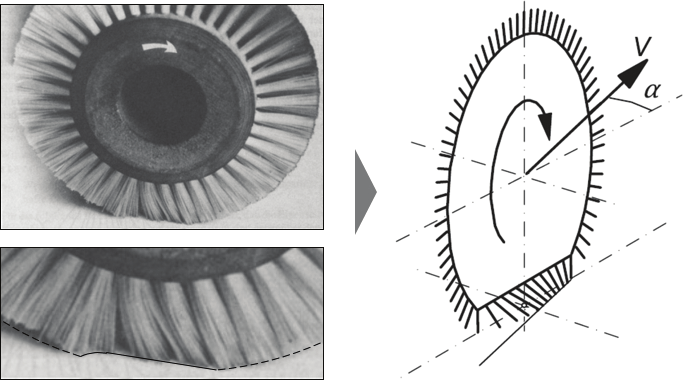
\includegraphics[width=0.5\linewidth]{../Figures/brush_model}
	\end{figure}
\end{frame}

\begin{frame}[fragile]
	\begin{center}
		\Huge{\textbf{FINE}}
	\end{center}
\end{frame}

% APPENDICI %%%%%%%%%%%%%%%%%%%%%%%%%%%%%%%%%%%%%%%%%%%%%%%%%%%%%%%%%%%%%%%%%%%%%%%%%%%%%%%%%%%

\begin{frame}[fragile]
	\begin{center}
		\huge{\textbf{Intersezione trà alberi di tipo AABB}}
	\end{center}
\end{frame}

\begin{frame}[fragile]
	\Large{\textbf{Intersezione trà alberi di tipo AABB}}
	\normalsize
	\\[0.2cm]
	Volendo intersecare due semplici AABB, quali:
	\begin{equation*}
	\begin{split}
	A = \left[ \texttt{A.minX}, \texttt{A.maxX},  \texttt{A.minY}, \texttt{A.maxY} \right]\\
	B = \left[ \texttt{B.minX}, \texttt{B.maxX},  \texttt{B.minY}, \texttt{B.maxY} \right]
	\end{split}
	\end{equation*}
	verrà usata la seguente funzione:
	\vspace{.8em}
	\begin{pseudoc}
function intersect(A,B) {
    return (A.minX <= B.maxX && A.maxX >= B.minX) &&
    (A.minY <= B.maxY && A.maxY >= B.minY)
}
\end{pseudoc}
\end{frame}

\begin{frame}[fragile]
	\begin{center}
		\huge{\textbf{Intersezione trà entità geometriche}}
	\end{center}
\end{frame}

\begin{frame}[fragile]
	\Large{\textbf{Intersezione segmento-punto}}
	\normalsize
	\\[0.2cm]
	Dato un punto $P = (x_p, y_p)$ e un segmento definito dai punti $A = (x_A, y_B)$ e $B = (x_B, y_B)$.
	\begin{figure}[h!]
		\centering
		\begin{tikzpicture}
		\def\r{2};
		\coordinate (P) at (0.3,0.7);
		\coordinate (A) at (-2.0,0.0);
		\coordinate (B) at (+2.0,0.0);
		\draw[fill] (A) circle [radius=1pt] node[above] {$A$};
		\draw[fill] (B) circle [radius=1pt] node[above] {$B$};
		\draw[fill] (P) circle [radius=1pt] node[above] {$P$};
		\draw[thick](A) -- (B);
		\end{tikzpicture}
	\end{figure}
	\noindent
	Per determinare se il punto $P$ è interno al segmento gli \textit{step} sono:
	\begin{enumerate}
		\item creazione di un vettore $\vec{AB}$ e di un vettore $\vec{AP}$;
		\item calcolo del prodotto vettoriale  $\vec{AB} \times  \vec{PA}$, se il modulo del vettore risultante è nullo allora il punto $P$ appartiene al segmento considerato;
		\item calcolo del prodotto scalare tra $\vec{AB}$ e $\vec{AP}$, se è nullo allora $P \equiv A$, se è pari al modulo di $\vec{AB}$ allora il $P \equiv B$, se è compreso tra 0 il modulo di $\vec{AB}$, allora il punto $P$ giace all'interno del segmento considerato.
	\end{enumerate}
\end{frame}

\begin{frame}[fragile]
	\Large{\textbf{Intersezione punto-cerchio}}
	\normalsize
	\\[0.2cm]
	Data una circonferenza con centro $C = (x_c, y_c)$ e raggio $r$, il problema consiste nel trovare se un generico punto $P = (x_p, y_p)$ è all'interno, all'esterno o corrispondente alla circonferenza.
	\begin{figure}[h]
		\centering
		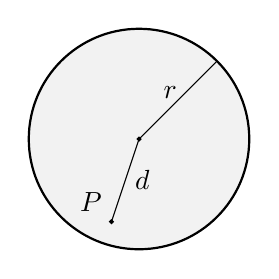
\begin{tikzpicture}[scale=0.7]
		\def\r{2};
		\coordinate (C) at (0,0) node[above left] {$C$};
		\draw[thick, fill=gray!10](C) circle (\r);
		\coordinate (P) at (-0.5,-1.5);
		\draw[fill] (C) circle [radius=1pt];
		\draw[fill] (P) circle [radius=1pt];
		\draw(C) -- (P)  node[above left] {$P$} node[pos=0.5, right] {$d$};
		\draw(C) -- ({sqrt(\r)},{sqrt(\r)}) node[pos=0.4, above] {$r$};
		\end{tikzpicture}
	\end{figure}
	La soluzione al problema è semplice: la distanza tra il centro della circonferenza $C$ e il punto $P$ è data dal teorema di Pitagora, ovvero:
	\begin{equation*}
	d=\sqrt{(x_p-x_c)^2 + (y_p-y_c)^2}
	\end{equation*}
\end{frame}

\begin{frame}[fragile]
	\Large{\textbf{Intersezione piano-piano}}
	\normalsize
	\\[0.2cm]
	\begin{figure}
		\centering
		\tdplotsetmaincoords{70}{110}
		\begin{tikzpicture}[tdplot_main_coords,font=\sffamily, scale= 0.7]
		\draw[-latex] (0,0,0) -- (4,0,0) node[left] {$x$};
		\draw[-latex] (0,0,0) -- (0,4,0) node[below] {$y$};
		\draw[-latex] (0,0,0) -- (0,0,4) node[left] {$z$};
		\tdplotsetrotatedcoords{45}{0}{0}
		\begin{scope}[tdplot_rotated_coords]
		\draw[fill=gray!10,opacity=0.6] (-3,0,-3) -- (-3,0,3) -- (3,0,3) -- (3,0,-3) -- cycle;
		\end{scope}
		\tdplotsetrotatedcoords{90}{45}{0}
		\begin{scope}[tdplot_rotated_coords]
		\draw[fill=gray!10,opacity=0.5] (-3,-3,0) -- (-3,3,0) -- (3,3,0) -- (3,-3,0) -- cycle;
		\draw[thick](-3,{3/sqrt(2)},0) coordinate(x) --(3,{-3/sqrt(2)},0);
		\end{scope}
		\node[anchor=south east,align=center] (line) at (3,-1.5,3.5) {$L$};
		\draw[-latex] (line) to[out=0,in=135] (x);
		\end{tikzpicture}
	\end{figure}
	\begin{equation*}
		L(s) = \frac{(d_2\vec{n}_1 - d_1\vec{n}_2) \times \vec{u}}{|\vec{u}|^2}+s\vec{u}
	\end{equation*}
\end{frame}

\begin{frame}[fragile]
	\Large{\textbf{Intersezione piano-segmento e piano-raggio}}
	\normalsize
	\\[0.2cm]
	\begin{figure}
		\centering
		\tdplotsetmaincoords{70}{110}
		\begin{tikzpicture}[tdplot_main_coords]
		\draw[-latex] (0,0,0) -- (4,0,0) node[left] {$x$};
		\draw[-latex] (0,0,0) -- (0,4,0) node[below] {$y$};
		\draw[-latex] (0,0,0) -- (0,0,4) node[left] {$z$};
		
		\draw[fill=gray!10,opacity=0.5] (-3,-3,0) -- (-3,3,0) -- (3,3,0) -- (3,-3,0) -- cycle;
		\draw[-stealth,thick] (0,-0.75,3.25) node[above] {$P_0$} -- (0,1.25,1.25) node[above right] {$P_1$};
		\draw (0,-0.5,2.25) node[below left] {$\vec{w}$};
		\draw (0,0.25,2.25) node[above right] {$\vec{u}$};
		\draw[-stealth,thick] (0,0,0) -- (0,-0.75,3.25);
		\draw[dashed] (0,1.25,1.25) -- (0,2.5,0);
		\draw[fill] (0,2.5,0) circle [radius=1pt];
		\draw (0,2.5,0) node[below left] {$P(t_I)$};
		\draw (0,2,0.5) node[right] {$P(t)$};
		\draw[fill] (0,2,.5) circle [radius=1pt];
		\draw[-stealth,thick] (1,-2,0) -- (1,-2,2) node[left] {$\vec{n}$};
		\end{tikzpicture}
	\end{figure}
	\begin{equation*}
	\vec{n} \cdot (\vec{w}+t\vec{u}) = 0
	\qquad
	t_I = -\frac{\vec{n}\cdot\vec{w}}{\vec{n}\cdot\vec{u}}
	\end{equation*}
\end{frame}

\begin{frame}[fragile]
	\Large{\textbf{Intersezione raggio-triangolo}}
	\normalsize
	\\[0.2cm]
\begin{figure}[htbp]
	\centering
	\hfill
	\begin{subfigure}[t]{.45\linewidth}
		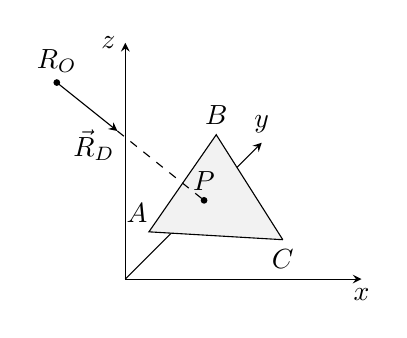
\begin{tikzpicture}
		\coordinate (O) at (0,0,0);
		\def\axisl{3}
		\draw[-stealth] (O) -- (\axisl,0,0) node[below]{$x$};
		\draw[-stealth] (O) -- ({sqrt(\axisl)},{sqrt(\axisl)},0) node[above]{$y$};
		\draw[-stealth] (O) -- (0,\axisl,0) node[left]{$z$};
		\coordinate [label=below:$C$] (V1) at ({\axisl/1.5},0.5,0);
		\coordinate [label=above:$B$] (V2) at ({sqrt(\axisl)/1.5},{3.3/1.8},0);
		\coordinate [label={[shift={(-0.15,0)}]$A$}] (V3) at (0.3,0.6,0);
		\draw[fill=gray!10] (V1) -- (V2) -- (V3) -- (V1);
		
		\def\xp{1};
		\def\yp{1};
		\def\xd{-1};
		\def\yd{0.8};
		\def\mag{1.7};
		\coordinate [label=above:$P$] (P) at (\xp,\yp);
		\coordinate [label={[shift={(-0.3,-0.5)}]$\vec{R}_D$}] (RD) at (\xp+\xd*1.1,\yp+\yd*1.1);
		\coordinate [label=above:$R_O$] (RO) at (\xp+\xd*\mag*1.1,\yp+\yd*\mag*1.1);
		\draw[fill] (P) circle [radius=1pt];
		\draw[fill] (RO) circle [radius=1pt];
		\draw[-stealth] (RO) -- (RD);
		\draw[dashed] (RD) -- (P);
		\end{tikzpicture}
	\end{subfigure}
	\hfill
	\begin{subfigure}[t]{.45\linewidth}
		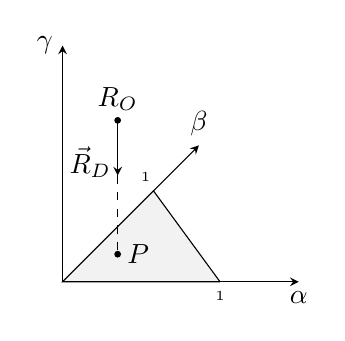
\begin{tikzpicture}
		\coordinate (O) at (0,0,0);
		\def\axisl{3}
		\draw[-stealth] (O) -- (\axisl,0,0) node[below]{$\alpha$};
		\draw[-stealth] (O) -- ({sqrt(\axisl)},{sqrt(\axisl)},0) node[above]{$\beta$};
		\draw[-stealth] (O) -- (0,\axisl,0) node[left]{$\gamma$};
		\coordinate [label={[below,font=\tiny]:$1$}] (V1) at ({\axisl/1.5},0,0);
		\coordinate [label={[shift={(-0.1,0.0)},font=\tiny]:$1$}] (V2) at ({sqrt(\axisl)/1.5},{sqrt(\axisl)/1.5},0);
		\coordinate (V3) at (0,0,0);
		\draw[fill=gray!10] (V1) -- (V2) -- (V3) -- (V1);
		
		\def\xp{0.7};
		\def\yp{0.35};
		\def\xd{0};
		\def\yd{1};
		\def\mag{1.7};
		\coordinate [label=right:$P$] (P) at (\xp,\yp);
		\coordinate [label={[shift={(-0.35,-0.15)}]$\vec{R}_D$}] (RD) at (\xp+\xd,\yp+\yd);
		\coordinate [label=above:$R_O$] (RO) at (\xp+\xd*\mag,\yp+\yd*\mag);
		\draw[fill] (P) circle [radius=1pt];
		\draw[fill] (RO) circle [radius=1pt];
		\draw[-stealth] (RO) -- (RD);
		\draw[dashed] (RD) -- (P);
		\end{tikzpicture}
	\end{subfigure}
	\hfill
\end{figure}
	\begin{equation*}
	R_O + t\vec{R}_D = A+u(B-A)+v(C-A)
	\end{equation*}
	\begin{equation*}
	\begin{bmatrix}
	t \\
	u \\
	v
	\end{bmatrix} 
	= \frac{1}{(D \times E_2) \cdot E_1}
	\begin{bmatrix}
	(T \times E_1) \cdot E_2 \\
	(D \times E_2) \cdot T \\
	(T \times E_1) \cdot D
	\end{bmatrix}
	= \frac{1}{P \cdot E_1}
	\begin{bmatrix}
	Q \cdot E_2 \\
	P \cdot T \\
	Q \cdot D
	\end{bmatrix}
	\end{equation*}
\end{frame}

\begin{frame}[fragile]
	\begin{center}
		\huge{\textbf{La libreria \texttt{TireGruond}}}
	\end{center}
\end{frame}

\tikzset{
	treenode/.style = {shape=rectangle, 
		draw, align=center, fill = gray!10},
	root/.style     = {treenode, font=\Large},
	env/.style      = {treenode, font=\ttfamily\normalsize},
	tt/.style      = {font=\ttfamily\normalsize},
	dummy/.style    = {circle,draw}
}

\begin{frame}[fragile]
	\Large{\textbf{\texttt{class Tire}}}
	\normalsize
	\\[0.2cm]
	\begin{figure}[h!]
		\centering
		\begin{tikzpicture}
		[
		grow                    = down,
		sibling distance    = 8em,
		level distance       = 8.5em,
		edge from parent/.style = {draw,-stealth},
		every node/.style       = {font=\footnotesize},
		sloped
		]
		\node [root, env] {Tire}
		child { node [env] {SamplingGrid}
			edge from parent node [below,tt] {Precision} }
		child { node [env] {ETRTO}
			edge from parent node [below,tt] {TireGeometry} }
		child { node [env] {Shadow}
			edge from parent node [below,tt] {TireShadow} }
		child { node [env] {ReferenceFrame}
			edge from parent node [below,tt] {RF} };
		\end{tikzpicture}
	\end{figure}
\end{frame}

\begin{frame}[fragile]
	\Large{\textbf{\texttt{class MagicFormula}}}
	\normalsize
	\\[-1cm]
	\begin{figure}[h!]
		\centering
		\begin{tikzpicture}
		[
		grow                    = down,
		sibling distance    = 8em,
		level distance       = 8.5em,
		edge from parent/.style = {draw,-stealth},
		every node/.style       = {font=\footnotesize},
		sloped
		]
		\node [root, env] {MagicFormula}
		child { node [env] {Tire}
			child { node [env] {SamplingGrid}
				edge from parent node [below,tt] {Precision} }
			child { node [env] {ETRTO}
				edge from parent node [below,tt] {TireGeometry} }
			child { node [env] {Shadow}
				edge from parent node [below,tt] {TireShadow} }
			child { node [env] {ReferenceFrame}
				edge from parent node [below,tt] {RF} }
			edge from parent node [below,tt] {} }
		child { node [env] {Disk}
			edge from parent node [below,tt] {SingleDisk} };
		\end{tikzpicture}
	\end{figure}
\end{frame}

\begin{frame}[fragile]
	\Large{\textbf{\texttt{class MultiDisk}}}
	\normalsize
	\\[-1cm]
	\begin{figure}[h!]
		\centering
		\begin{tikzpicture}
		[
		grow                    = down,
		sibling distance    = 8em,
		level distance       = 8.5em,
		edge from parent/.style = {draw,-stealth},
		every node/.style       = {font=\footnotesize},
		sloped
		]
		\node [root, env] {MultiDisk}
		child { node [env] {Tire}
			child { node [env] {SamplingGrid}
				edge from parent node [below,tt] {Precision} }
			child { node [env] {ETRTO}
				edge from parent node [below,tt] {TireGeometry} }
			child { node [env] {Shadow}
				edge from parent node [below,tt] {TireShadow} }
			child { node [env] {ReferenceFrame}
				edge from parent node [below,tt] {RF} }
			edge from parent node [below,tt] {} }
		child { node [env] {Disk}
			edge from parent node [below,tt] {DiskVec} };
		\end{tikzpicture}
	\end{figure}
\end{frame}

\end{document}